\documentclass[12pt]{article}        % Classe de document: rapport

\usepackage[french]{babel}          % Langue du document: français
\usepackage[utf8]{inputenc}         % Encodage du document: UTF-8
\usepackage[T1]{fontenc}            % Encodage des polices: T1 
\usepackage{fancybox}               % Boîtes de texte stylisées
\usepackage{hyperref}               % Liens hypertexte
\usepackage{color}                  % Couleurs
\usepackage{setspace}               % Interligne
\usepackage{graphicx}               % Images
\usepackage{float}                  % For [H] float placement

\begin{document}                    % Début du document

% PAGE DE GARDE
\begin{titlepage}
    \centering

    \Huge\textbf{ZayLou Games}\\
    \LARGE Créer son propre jeu sans coder\\[2cm]

    \textbf{Lallia Diakité: 20256054 \\
     Marc Olivier Jean Paul: 20241763} \\[2cm]

    IFT3150 - Projet d'informatique - Été 2025\\[2cm]

    \textbf{Superviseur :} Louis-Édouard Lafontant\\[2cm]

    Département d’informatique et de recherche opérationnelle\\[1cm] 
    Université de Montréal\\[1cm]

    \vfill

    {\large Date : \today}
\end{titlepage}

% TABLE DES MATIÈRES
\tableofcontents                    % Génération de la table des matières
\newpage                            % Nouvelle page


\section{Introduction}              
\label{sec:introduction}       
Ce document présente les avancées faites dans le projet \textbf{ZayLou 
Games}, dans le cadre du cours IFT3150 - Projet d'informatique de 
l'Université de Montréal à l'été 2025.

\subsection{Contexte}               
\label{subsec:contexte}             
Si de nos jours, plusieurs plateformes permettent de créer des 
jeux-vidéos sans avoir à écrire du code, beaucoup d'entre elles sont 
assez compliquées à prendre en main. Pour le reste, elles sont souvent 
limitées en termes de fonctionnalités: elles ne permettent pas 
l'interaction physique dans le jeu.

Certaines technologies permettent les interactions physiques dans les 
jeux-vidéos, mais ne sont pas très connues ou utilisées. Il serait donc 
intéressant de pouvoir les utiliser lors d'une partie de jeu, afin de 
rendre l'expérience de jeu plus immersive et interactive.

\subsection{Problématiques et motivations}               
\label{subsec:Problématiques et motivations}          
Même avec le grands nombre de plateformes de création de jeux-vidéos
disponibles, il est difficile de trouver une plateforme qui soit:
\begin{itemize}
    \item Simple à prendre en main, sans avoir à écrire de code;
    \item Permettant de créer des jeux-vidéos avec des interactions 
    physiques;
    \item Accessible à tous, sans avoir à passer par des étapes 
    compliquées
    ou des configurations complexes.
\end{itemize}
Ce sont ces problématiques qui nous ont incités à travailler sur 
\textbf{ZayLou Games}. Notre motivations est de permettre à tout le monde 
de créer son propre jeu-vidéo sans avoir à écrire de code, tout en 
apportant une couche d'originalité avec les interactions physiques.

\subsection{Objectifs}             
\label{subsec:objectifs}             
Avec \textbf{ZayLou Games}, nous avons pour objectif de permettre à tout 
le monde de créer son propre jeu-vidéo en 2D sur une plateforme web 
intuitive, de jouer au jeu créé à l'aide d'une application mobile, et 
d'utiliser la technologie NFC pour permettre des interactions physiques 
dans le jeu.

\newpage                            

\section{Analyse des besoins et étude préliminaire}              
\label{sec:Analyse}                                              
Comme pour tout projet, il est important de commencer par une analyse 
des besoins et une étude préliminaire. Nous avons donc passé plusieurs 
semaines à itérer sur les besoins du projet.

\subsection{Exigences fonctionnelles et non-fonctionnelles}              
\label{subsec:Exigences}          
Voici la liste des exigences que la plateforme doit supporter:

\subsubsection{Exigences fonctionnelles}
\label{subsubsec:fonctionnelles}  
L'utilisateur doit pouvoir créer un jeu simple. Lors de la création,
il doit pouvoir donner un nom, une description et une catégorie au jeu,
sélectionner une ou plusieurs cases de la grille pour définir des éléments
dans le jeu (comme la position de départ du joueur, les pièges, etc).
L'utilisateur doit aussi pouvoir ajuster les dimensions des objets définis 
dans la grille, et ajouter des conditions logiques pour enrichir la 
dynamique du jeu. Il peut aussi cumuler des effets jusqu'à un certain 
point, et même superposer des effets (par exemple, appliquer plusieurs 
effets en même temps).

Il faut aussi que l'utilisateur ait la possibilité de consulter tous 
les jeux qu'il a créés. Il doit pouvoir y jouer à l'aide
de l'application mobile. Il pourra également scanner une carte NFC,
pour déclencher un effet associé dans le jeu.

La plateforme web doit fournir à l'utilisateur une grille interactive
pour la création de son jeu. La grille sera composée de cases qui 
devront permettre à l'utilisateur de définir ses éléments de jeu.
La plateforme doit aussi permettre à l'utilisateur non seulement de créer 
les effets qu'il veut mettre dans son jeu, mais aussi de les sauvegarder
pour les réutiliser dans d'autres jeux. Il est aussi important que la 
plateforme web permette à l'utilisateur de sauvegarder son avancée dans 
la création de son jeu de manière à ce qu'il puisse récupérer l'état de 
la grille tel qu'il l'avait laissé avant la sauvegarde.

Quant à l'application mobile, elle doit pouvoir authentifier l'utilisateur
et synchroniser ses jeux avec le backend de manière à ce qu'il puisse les
retrouver. Une autre exigence fonctionnelle serait d'interpréter et 
d'évaluer les conditions logiques pour déclencher les effets selon le 
contexte du jeu. Il faut aussi que l'utilisateur puisse scanner les 
cartes NFC et que l'application extraie l'identifiant et déclenche en 
temps réel l'effet correspondant dans la session de jeu.

\subsubsection{Exigences non fonctionnelles}
\label{subsubsec:non fonctionnelles}  
Le processus de création de jeu doit être simple et intuitif, même
pour un utilisateur non expérimenté. Il doit aussi être conçu pour 
éviter toute complexité excessive: l'utilisateur doit clairement
savoir où aller pour avoir ce qu'il veut, même à la première utilisation.
L'ajout de nouveaux effets doit être fluide et rapide, sans nécessiter de
connaissances techniques avancées. L'interface utilisateur doit rester
ergonomique, même avec un grand nombre d'éléments dans le jeu.

Les données échangées entre l'application (mobile/web) et le backend
doivent être chiffrées et protégées contre les interceptions
(en utilisant l'authentification par JWT par exemple). Les requêtes API
doivent être protégées contre les accès non autorisés. Il fuadra donc 
toujours faire une vérification de l'identité de l'utilisateur et 
contrôler les droits d'accès aux ressources.

La plateforme mobile doit être conçue pour être compatible avec les 
systèmes IOS et Android. Il faut aussi que chaque composant logiciel
(API, interface, etc.) soit testable indépendamment de manière à
faciliter les tests unitaires et les tests d'intégration. Le système doit
pouvoir supporter l'ajout fréquent de nouveaux jeux ou effets sans 
dégradation notable des performances. 

\subsection{Méthodologie utilisée}
\label{Méthodologie}
Nous avons décidé d'utiliser la méthodologie Agile pour le développement 
de la plateforme. Cette méthodologie nous permet de travailler de manière 
itérative et incrémentale, ce qui est idéal pour un projet de cette 
envergure. Nous avons donc commencé par définir les exigences 
fonctionnelles et non-fonctionnelles, puis nous avons continué avec le 
prototype figma de la plateforme web.

Nous avions aussi organisé des réunions hebdomadaires avec le Superviseur pour discuter de l'avancement
du projet et des problèmes rencontrés. Pour le développement, nous avons utilisé GitHub pour
gérer le code source et les versions du projet. Vu que nous sommes deux dans le projet,
côté implémentations, l'un de nous s'est occupé de la partie backend et l'autre de la partie frontend.

\subsection{Étude de solutions similaires ou existantes}
\label{Étude de solutions}
Il existe plusieurs plateformes qui permettent de créer des jeux-vidéos sans avoir à écrire de code.
Parmi elles, on peut citer: \textbf{Scratch}, \textbf{Unity Playground}, \textbf{Gamefroot}, etc. 
Nous avons fait quelques recherches, regarder quelques vidéos pour comprendre comment fonctionnent 
ces plateformes, et c'est à partir de là que nous sommes arrivées à la conclusion que la plupart de 
ces plateformes sont assez complexes à prendre en main. De plus, même si elles présentent de nombreuses 
fonctionnalités, certaines de ces dernières ne sont pas évidentes à trouver, ce qui contribue à diminuer 
l'efficience du processus de création.

Autre point important, la plupart de ces plateformes ne donnent pas à l'utilisateur une liberté totale:
En effet, l'utilisateur ne peut qu'utiliser les objets prédéfinis par la plateforme, et ne peut pas
ajouter de nouveaux objets ou effets. 

C'est donc en partant de ce constat que nous nous sommes mis à chercher des innovatoions à apporter
à la plateforme. Nous avons donc décidé que l'utilisateur doit pouvoir créer et ajouter ses 
propres effets au jeu, et que la plateforme doit permettre des interactions physiques avec le scan des
cartes NFC.

\section{Conception}
\label{sec:Conception}             
La conception de la plateforme a été faite en plusieurs étapes.
Nous avons commencé par définir l'architecture de la plateforme, puis nous avons créé un prototype figma
de la plateforme web. Ensuite, nous avons commencé à implémenter la plateforme en utilisant les technologies
les plus adaptées à nos besoins.

\subsection{Architecture du système}
\label{subsec:Architecture}
Voici le diagramme de l'architecture du système:
\begin{figure}[H]
    \centering
    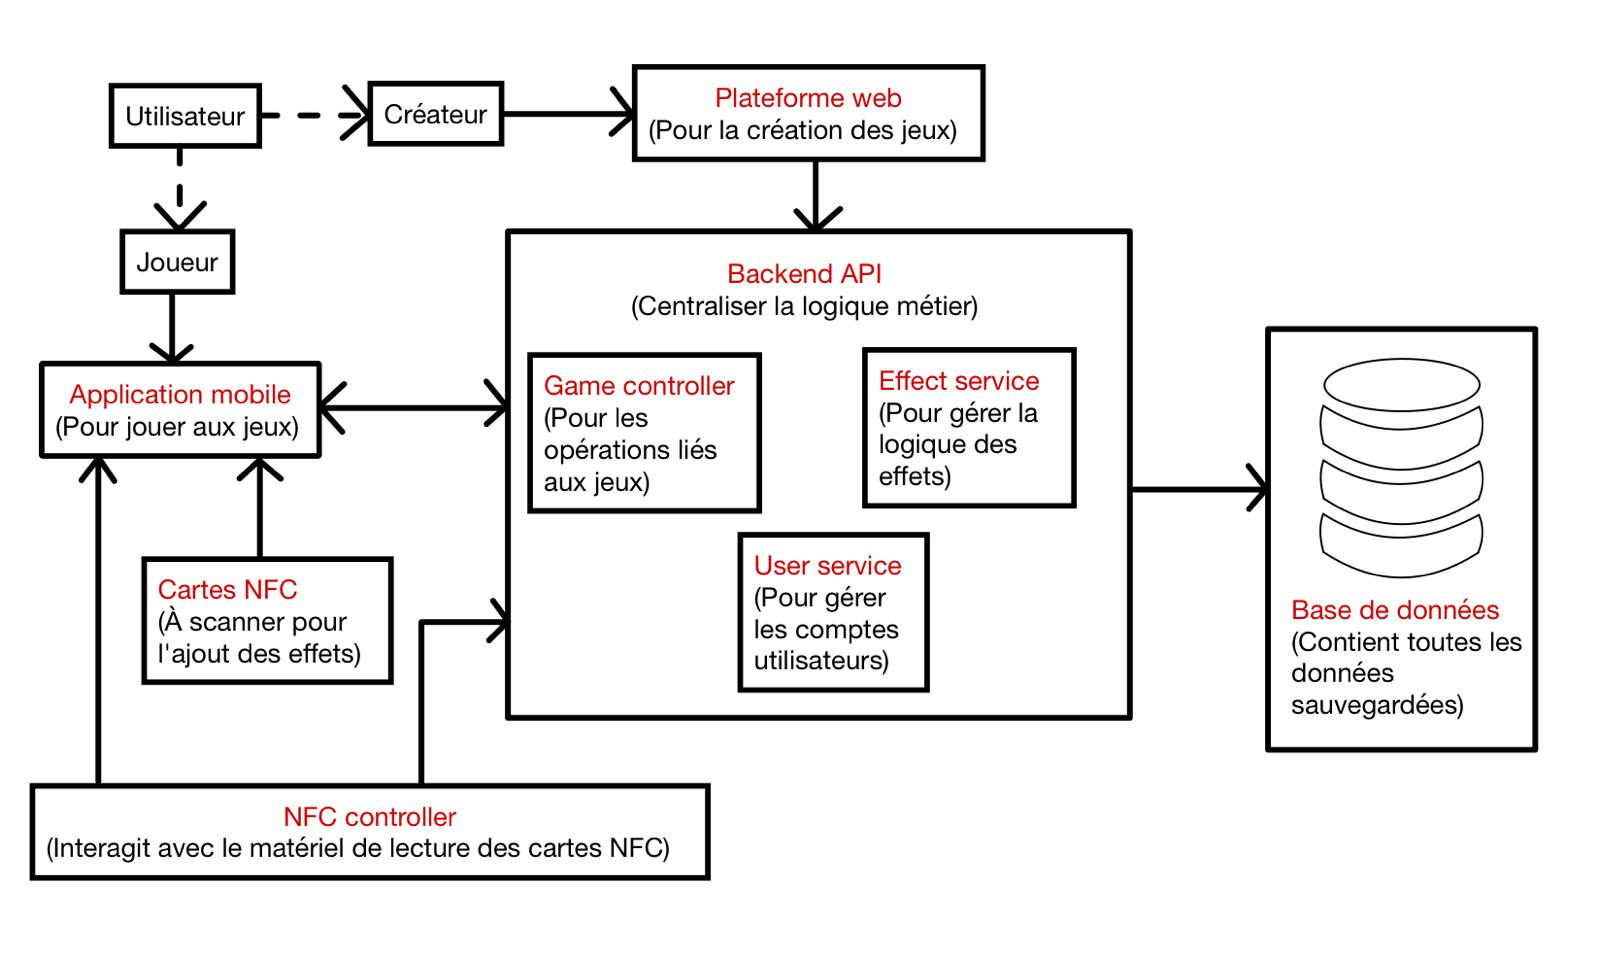
\includegraphics[width=\textwidth]{diagrammeC4.jpg}
    \caption{Diagramme C4 de l'architecture du système}
    \label{fig:diagramme C4}
\end{figure} 

L'architecture du projet est basée sur une séparation claire entre les 
différentes couches de la plateforme, assurant une bonne organisation des
responsabilités. 

L'utilisateur peut adopter deux rôles distincts:
En tant que créateur, il interagit avec la plateforme web pour concevoir, 
sauvegarder et configurer ses jeux. Cette plateforme envoie des 
requêtes HTTP vers le Backend API, qui centralise les opérations côté 
serveur.

Ensuite, en tant que joueur, il utilise l'application mobile pour jouer
aux jeux déjà créés et intéragir avec des cartes physiques via la 
technologie NFC. L'application mobile, permettra aux joueurs 
de jouer à leurs jeux, de scanner des cartes NFC à l'aide d'un 
NFC Controller et de synchroniser les états du jeu avec le backend 
via des requêtes API.

Lorsqu'une carte NFC est scannée, le NFC Controller lit son identifiant, 
qui est ensuite envoyé au backend via l'application mobile. Le backend 
identifie alors l’effet associé et l’applique via le Effect Service.

Le Backend API centralise toute la logique métier. Il reçoit les 
requêtes de la plateforme web ou de l'application mobile, et se charge
de l'enregistrement et de la récupération des jeux via le GameController,
de l'application des effets dynamiques via l'Effect Service et de la 
gestion des comptes utilisateurs avec le User Service.
Toutes les données persistantes sont stockées dans une base de données
reliée directement au Backend.

\subsection{Modèle de données}
\label{subsec:modèle de données}
Le modèle de données du système repose sur une architecture orientée 
objet et un stockage en base de données NoSQL. Les données échangées 
avec le frontend et le backend sont transformées en JSON. Cela facilitera
leur intégration dans les requêtes API et leur stockage dans la base de 
données.

\subsubsection{Structure et entités principales}
\label{subsubsec:structure et entités principales}
Le système définit plusieurs entités principales, voici le diagramme qui
le montre clairement:
\begin{figure}[H]
    \centering
    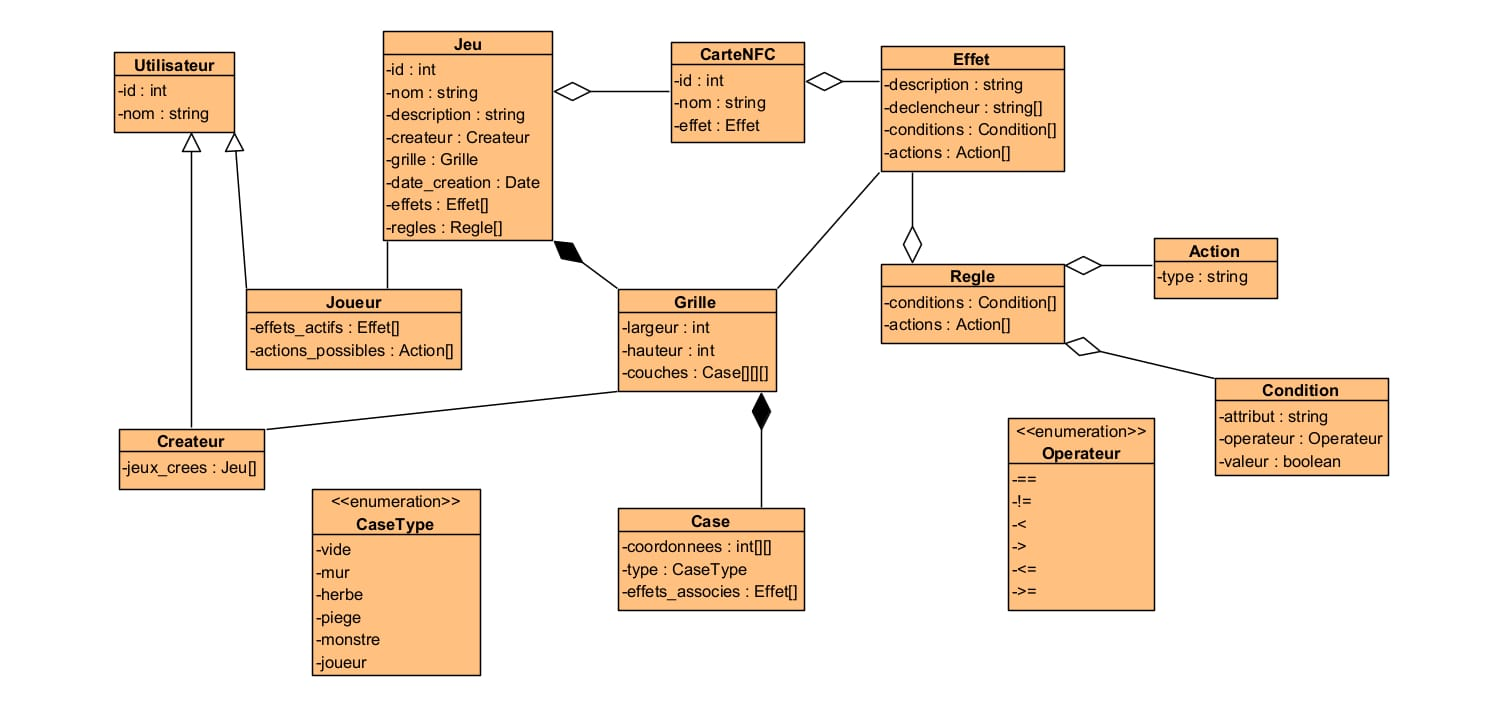
\includegraphics[width= \textwidth]{relation.jpg}
    \caption{Diagramme de classes du système}
    \label{fig:diagramme de classes}
\end{figure}

\newpage

\begin{itemize}
    \item \textbf{Jeu} : représente un jeu créé par un utilisateur. Il 
    contient un \texttt{id}, un \texttt{nom}, une \texttt{description}, 
    un \texttt{créateur}, une \texttt{grille} pour construire le jeu , 
    une \texttt{date de création},  une liste d'\texttt{effets}, et un 
    ensemble de \texttt{règles}.

    \item \textbf{Grille} : représente la structure de jeu définie par 
    l'utilisateur. Elle possède une \texttt{largeur}, une 
    \texttt{hauteur}, et des \texttt{couches} qui sont des ensembles de 
    \texttt{cases}. Chaque case peut contenir un \texttt{élément} 
    (joueur, NPC, objet) et des \texttt{effets}.

    \item \textbf{Case} : représente une case de la grille, avec des 
    attributs comme les \texttt{coordonnées}, le \texttt{type} de
    la case et les \texttt{effets} associés. Le type de la case signifie 
    son rôle dans le jeu (vide, piège, obstacle, etc.).

    \item \textbf{CartNFC} : représente un élément NFC scannable, avec 
    un \texttt{id}, un \texttt{nom} et un \texttt{effet}.
  
    \item \textbf{Effet} : décrit une action déclenchée dans le jeu, 
    avec un \texttt{déclencheur} (déplacement, interaction...), 
    des \texttt{conditions} à vérifier et des \texttt{actions} 
    à exécuter. Chaque effet possède ausi une \texttt{description}.

    \item \textbf{Utilisateur} : Représente toute personne utilisant soit
    l'application mobile, soit la plateforme web. Il possède un 
    \texttt{id} et un \texttt{nom}.
  
    \item \textbf{Joueur} : Une spécialisation de l'utilisateur. Il 
    représente celui qui utilise l'application mobile. Il possède en plus 
    des attributs de l'utilisateur, les effets actifs et les actions
    possibles dans le jeu.

    \item \textbf{Créateur} : Une autre spécialisation de l'utilisateur.
    Il s'agit de l'utilisateur qui utilise la plateforme web pour créer
    un jeu. Il possède comme attributs, ceux de l'utilisateur et ses jeux 
    créés.
  
    \item \textbf{Action} : Représente les actions que le joueur peut 
    accomplir dans son jeu.

    \item \textbf{Condition} : Permet de vérifier si un effet où une 
    règle doit être déclenché.

    \item \textbf{Règle} : Décrit des comportements généraux du jeu
\end{itemize}

\subsection{Choix technologiques: justifications, contraintes 
et alternatives}
\label{subsec:Choix technologiques}
Pour le développement de la plateforme, nous avons choisi de partir 
sur la division suivante:

\subsubsection{Frontend}
\label{subsubsec:Frontend}
Pour le frontend, nous avons décidé d'utiliser React. Il s'agit 
d'un framework très populaire et facile à prendre en main. 
React est idéal pour ce projet car il permet de créer des interfaces 
utilisateur dynamiques et réactives, ce qui répond parfaitement
aux besoins du projet. En effet, la plateforme web comporte une
grille avec lqauelle l'utilisateur intéragira pour créer son jeu.
C'est donc pour cela que React est une bonne option.

\subsubsection{Backend}
\label{subsubsec:Backend}
Pour le backend, c'est avec Node.js avec Express.js que nous avons
décidé de travailler. Node.js est une plateforme JavaScript côté serveur 
qui permet de créer des applications web performantes et scalables.
Express.js quant à lui est un framework minimaliste pour Node.js qui 
facilite la création d'API REST.
Node.js est très prisé pour les applications en temps réel et avec
beaucoup d'entrées/sorties. De son côté, Express.js facilite la gestion
requêtes et la création des routes. Tout ceci montre pourquoi Node.js et 
Express.js sont de bons choix pour ce projet.

\subsubsection{Base de données}
\label{subsubsec:Base de données}
Pour la base de données, nous avons choisi d'utiliser MongoDB.
MongoDB est une base de données NoSQL orientée document qui permet 
de stocker des données sous forme de JSON. Elle est très flexible et 
permet de stocker des données de manière non structurée, ce qui est idéal 
pour notre projet. De plus, MongoDB est très performante et permet de 
gérer de grandes quantités de données facilement.

\subsection{Prototype ou maquette de l’interface}
\label{subsec:Prototype}
Pour la conception de l'interface utilisateur, nous avons utilisé Figma 
pour créer un prototype interactif de la plateforme web. Le prototype 
permet de visualiser l'interface utilisateur, les différentes pages et 
les interactions possibles. Voici le lien vers le prototype 
Figma: \href{https://www.figma.com/design/eKXFDHbDRlhK4KngvE7KGb/
ZayLou_Games?node-id=0-1&t=n9lvoJhYaFOCaRAi-1}{ZayLou Figma}

\newpage                            % Nouvelle page

\section{Implémentation / Réalisation technique}
\label{sec:Implémentation}
L'implémentation de la plateforme a été faite en plusieurs étapes.
Nous avons commencé par mettre en place l'architecture du projet, 
puis nous avons implémenté le backend, la base de données, le frontend, 
le tout en parallèle. Cependant, nous nous sommes beaucoup concentrés 
sur le backend, car c'est lui qui gère la logique du jeu  et les 
interactions avec la base de données. De ce fait, il est beaucoup 
plus complet que le frontend, qui est encore en cours de développement.

\subsection{Présentation synthétique de l’implémentation}
\label{subsec:Présentation synthétique}
L’implémentation repose sur une architecture MERN: le frontend en React 
permet de manipuler la grille en temps réel, le backend en 
Node.js et Express expose une API REST, et les données sont stockées dans 
MongoDB via Mongoose. Les communications se font par des requêtes HTTP. 
Les principales fonctionnalités déjà en place incluent l’édition 
dynamique de la grille pour le frontend et l'exécution des requêtes
et les appels à la base de données pour le backend.

\subsection{Particularités vis-à-vis de la conception et autre 
contraintes}
\label{subsec:Particularités}
L’une des particularités de la conception a été de générer des
identifiants numériques uniques plutôt que d’utiliser les ObjectId 
MongoDB par défaut, afin d’offrir une meilleure lisibilité et gestion 
côté client et surtout car MongoDB ne fournit pas l'auto-incrémentation
des IDs. Le projet a aussi dû respecter certaines contraintes 
pédagogiques imposées (architecture MERN, API REST), et nous avons dû 
gérer cela dans un délai serré.

\subsection{Flux principaux}
\label{subsec:Flux principaux}
Nous avions fait un diagramme de séquence qui montre comment se déroule 
l'ajout des effets dans le jeu. Ce diagramme montre les différentes 
étapes du processus, depuis le scan de la carte NFC jusqu'à l'application 
de l'effet dans le jeu:

\newpage
\begin{figure}[H]
    \centering
    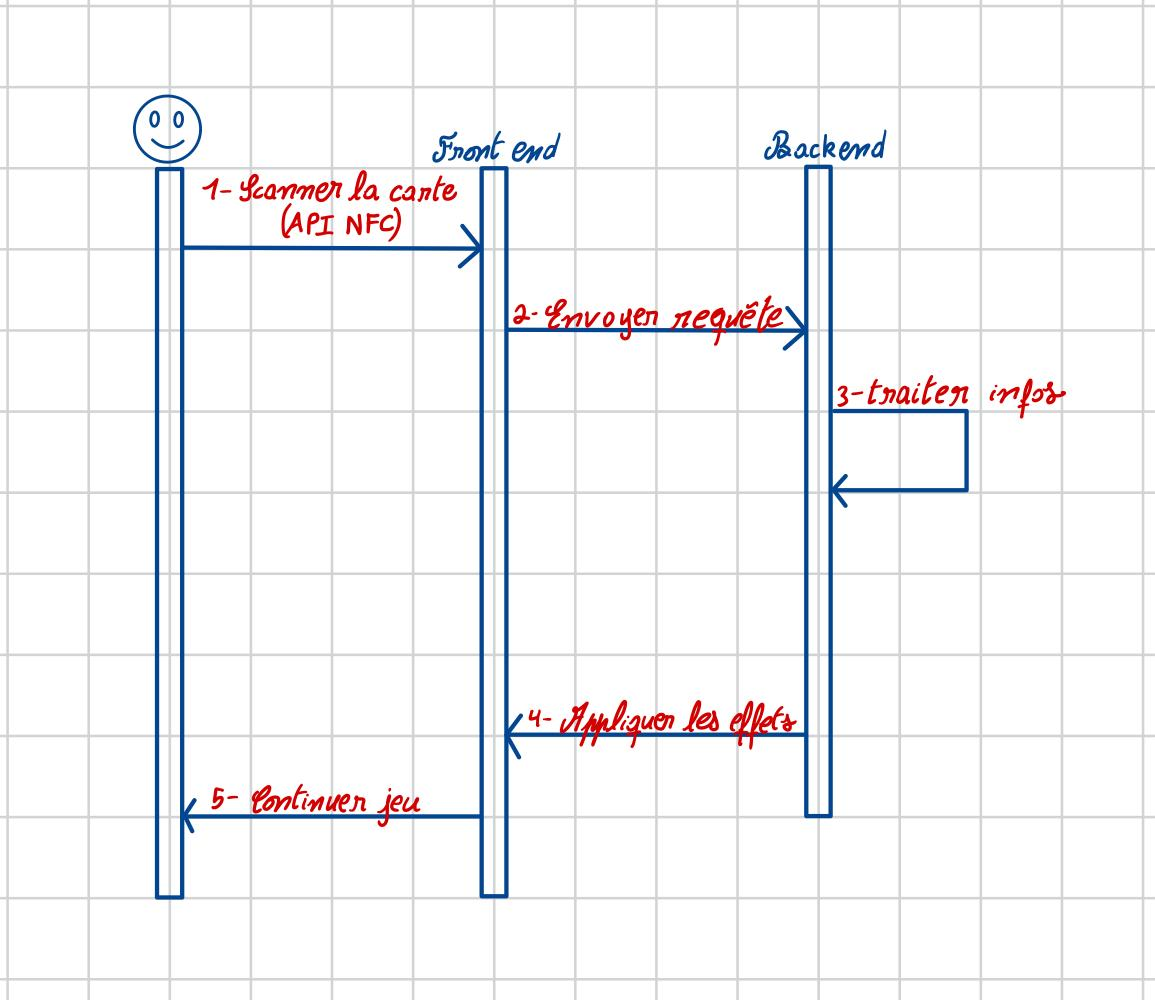
\includegraphics[width=\textwidth]{sequence.jpg}
    \caption{Diagramme de séquence pour l'application des effets}
    \label{fig:sequence effet}
\end{figure}

Lorsque l'utilisateur scanne la carte, Le frontend récupère les 
informations de la carte et envoie une requête HTTP vers le backend pour 
transmettre les données scannées. Le backend reçoit la requête et traite 
les informations : il peut identifier le type de carte, rechercher les 
effets associés, mettre à jour l’état du jeu, etc. Ensuite, il renvoie 
une réponse au frontend contenant les effets à appliquer. Le frontend 
applique les effets visuellement (changements d’état dans le jeu), 
puis le joueur continue à jouer avec le nouveau contexte.

\vspace{1cm}

Voici un autre diagramme de séquence qui montre comment se passe la 
sauvegarde d'un jeu dant le système:

\newpage
\begin{figure}[H]
    \centering
    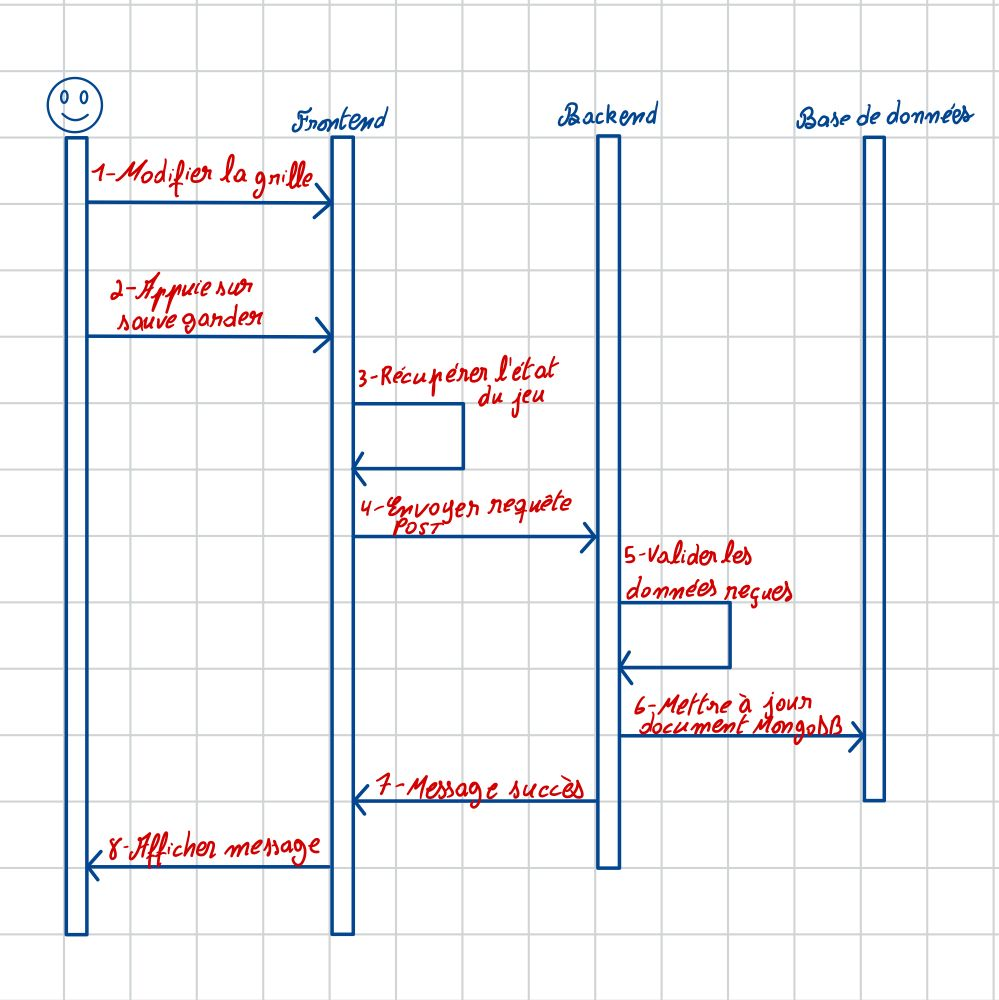
\includegraphics[width=\textwidth]{saveJeu.jpg}
    \caption{Diagramme de séquence pour la sauvegarde d'un jeu}
    \label{fig:sequence-sauvegarder}
\end{figure}

Une fois que l'utilisateur appuie sur sauvegarder après avoir modifié 
la grille, Le frontend récupère alors l’état actuel du jeu (grille, 
effets, règles, etc.) et l’envoie au backend via une requête HTTP POST.
Le backend reçoit cette requête, valide les données reçues pour s'assurer 
de leur cohérence, puis transmet la commande de mise à jour à la base de 
données MongoDB. Une fois la sauvegarde effectuée avec succès, le backend
renvoie un message de confirmation au frontend, qui se charge alors 
d’afficher un message de succès à l’utilisateur, l’informant que le jeu a 
bien été enregistré.

\subsection{Description détaillée des composants principaux}
\label{subsec:Description composants}
L’implémentation backend repose sur une séparation claire en couches : 
\begin{itemize}
    \item \textbf{Modèles et schémas Mongoose} : définissent la structure des entités necessaire en base MongoDB (ex. \texttt{Jeu}, \texttt{Utilisateur}, \texttt{Effet}, \texttt{CarteNFC}). 
    Les schémas imposent les types, les relations et certaines validations.
    \item \textbf{Services} : contiennent la logique métier.
    \begin{itemize}
        \item \texttt{JeuService} : gère la création, la récupération, la mise à jour et la suppression de jeux. Implémente la logique de sauvegarde en base et la génération d’identifiants numériques uniques via \texttt{genererIdUnique.ts} et \texttt{getNextId.ts}.
        \item \texttt{UtilisateurService} : gère l’inscription, l’authentification et la récupération des données utilisateur. Utilise \texttt{bcrypt} pour le hachage des mots de passe et \texttt{jsonwebtoken} pour la génération et la vérification des tokens.
        \item \texttt{EffetService} : s’occupe de la création et de la gestion des effets dans un jeu (déclencheurs, conditions, actions).
        \item \texttt{CarteNFCService} : gère l’association entre une carte NFC scannée et un effet à déclencher dans un jeu.
    \end{itemize}
    \item \textbf{Contrôleurs} : reçoivent les requêtes HTTP, valident les données entrantes et délèguent aux services.
    \begin{itemize}
        \item \texttt{jeuControllers.ts} : mappe les requêtes liées aux jeux vers les méthodes du \texttt{JeuService}.
        \item \texttt{utilisateurController.ts} : traite l’inscription, le login et la récupération d’informations utilisateur.
    \end{itemize}
    \item \textbf{Routes} : définies dans \texttt{jeuRoutes.ts} et \texttt{utilisateurRoutes.ts}, elles exposent les endpoints REST aux clients.
    \item \textbf{Middlewares} :
    \begin{itemize}
        \item \texttt{AuthMiddleware.ts} : vérifie la présence et la validité d’un token JWT pour protéger certaines routes.
        \item \texttt{validateEffetMiddleware.ts} : valide les données reçues lors de la création ou modification d’un effet.
    \end{itemize}
    \item \textbf{Utilitaires} :
    \begin{itemize}
        \item \texttt{genererIdUnique.ts} et \texttt{getNextId.ts} : gèrent la génération d’identifiants numériques uniques,
         en alternative aux \texttt{ObjectId} de MongoDB.
    \end{itemize}
\end{itemize}

Cette organisation modulaire permet de séparer les responsabilités, de faciliter la maintenance et d’étendre le projet
 en ajoutant de nouvelles fonctionnalités (par exemple de nouveaux types d’effets ou de règles) sans impacter le reste du système.



\section{Évaluation}
\label{sec:Evaluation}

\subsection{Tests unitaires et fonctionnels réalisés}
\label{subsec:Tests}
Les tests ont ciblé en priorité le cycle complet d’authentification ainsi que la persistance automatique côté client, car ce sont des fonctionnalités critiques dans le fonctionnement actuel de la plateforme.
\begin{itemize}
    \item \textbf{Inscription (\texttt{POST /api/utilisateurs})} : vérification de la création d’un compte avec les champs \texttt{nom}, \texttt{email} et \texttt{motDePasse}. Scénarios testés :
    \begin{itemize}
      \item création valide $\rightarrow$ code HTTP 201 et retour d’un objet utilisateur sans le mot de passe ;
      \item tentative avec un email déjà existant $\rightarrow$ code HTTP 409 ;
      \item schéma invalide (champs manquants ou format incorrect) $\rightarrow$ code HTTP 422.
    \end{itemize}
    
    \item \textbf{Connexion (\texttt{POST /login})} : validation de la génération d’un \textbf{JWT} signé à partir d’identifiants valides. Cas testés :
    \begin{itemize}
      \item connexion valide $\rightarrow$ code HTTP 200 et présence d’un champ \texttt{token} non vide ;
      \item mot de passe incorrect $\rightarrow$ code HTTP 401 ;
      \item utilisateur inexistant $\rightarrow$ code HTTP 404.
    \end{itemize}

    \item \textbf{Accès protégé (\texttt{GET /profils/\{id\}})} : contrôle que les routes protégées nécessitent bien un \texttt{Authorization: Bearer <token>} valide.
    \begin{itemize}
      \item accès par l’utilisateur lui-même ou un administrateur $\rightarrow$ code HTTP 200 ;
      \item accès par un autre utilisateur $\rightarrow$ code HTTP 403 ;
      \item absence ou expiration du token $\rightarrow$ code HTTP 401.
    \end{itemize}
    
    \item \textbf{Sauvegarde automatique de la grille} : côté frontend, toute modification du tableau de types (\texttt{state types}) déclenche une requête \texttt{PATCH /api/jeux/\{id\}} après un délai d’environ 500 ms (mécanisme de \textit{debounce}).
    \begin{enumerate}
      \item Modification unique $\rightarrow$ 1 requête \texttt{PATCH}.
      \item Série de modifications rapprochées $\rightarrow$ 1 seule requête regroupée (vérifiée via compteur d’appels).
      \item Perte de réseau temporaire $\rightarrow$ la sauvegarde reprend automatiquement au prochain changement ; cohérence vérifiée par relecture via \texttt{GET /api/jeux/\{id\}}.
    \end{enumerate}
  \end{itemize}
  \vspace{0.5em}
\noindent\textbf{Exemple de commandes utilisées pour tester} :

\begin{verbatim}
# Inscription
curl -X POST http://localhost:3000/api/utilisateurs \
 -H "Content-Type: application/json" \
 -d '{ "nom":"Test", "email":"docu@example.com", "motDePasse":"Secret123" }'

# Connexion -> récupère le token
TOKEN=$(curl -s -X POST http://localhost:3000/login \
 -H "Content-Type: application/json" \
 -d '{ "email":"docu@example.com", "motDePasse":"Secret123" }' | jq -r .token)

# Profil protégé
ID="<remplacer_par_id_utilisateur>"
curl http://localhost:3000/profils/$ID -H "Authorization: Bearer $TOKEN"
\end{verbatim}


\subsection{Évaluation de performance}
\label{subsec:performance}
Les mesures de performance ont été effectuées directement depuis l’outil de développement du navigateur (onglet Réseau apres avoir cliquer sur inspecter la page), en observant le temps de réponse des requêtes HTTP lors d’un usage normal.

\begin{itemize}
  \item \textbf{Inscription (\texttt{POST /api/utilisateurs})} : temps de réponse moyen observé $\approx$ 120\,ms. Les pics enregistrés (jusqu’à 200\,ms) sont apparus uniquement lors de la première requête après un démarrage du serveur.
  
  \item \textbf{Connexion (\texttt{POST /login})} : temps moyen $\approx$ 100\,ms. Même sous plusieurs tentatives consécutives, le temps est resté stable et inférieur à 150\,ms. Le token JWT est généré et renvoyé sans latence notable.
  
  \item \textbf{Accès profil protégé (\texttt{GET /profils/\{id\}})} : réponse en $\approx$ 90–110\,ms, incluant la vérification du JWT côté serveur.
  
  \item \textbf{Sauvegarde automatique de la grille (\texttt{PATCH /api/jeux/\{id\}})} : lors de modifications isolées, la requête prend en moyenne 130–140\,ms pour être traitée et confirmée. Avec plusieurs modifications rapprochées, 
  le mécanisme de \emph{debounce} regroupe les changements et n’envoie qu’une seule requête, réduisant l’impact sur la bande passante et maintenant la latence sous 150\,ms.
\end{itemize}

\noindent Ces temps ont été relevés dans un environnement local de développement, sans latence réseau significative.  
En conditions réelles (déploiement distant), on peut s’attendre à des temps légèrement supérieurs, mais la structure actuelle du backend et la taille réduite des payloads JSON permettent de rester dans des valeurs confortables ($<$ 200\,ms pour les opérations critiques).


\subsection{Évaluation d'utilisabilité}
\label{subsec: utilisabilité}

L’évaluation de l’utilisabilité s’est faite en observant l’expérience utilisateur globale lors de scénarios typiques (inscription, connexion, modification de grille) et en vérifiant la clarté des interactions.

\begin{itemize}
  \item \textbf{Visibilité de l’état du système} : l’utilisateur reçoit un retour visuel après les actions importantes (confirmation après sauvegarde automatique de la grille, redirection vers son espace après connexion réussie). Les temps de réponse sont courts, ce qui renforce la perception de fluidité.
  
  \item \textbf{Correspondance entre le système et le monde réel} : les libellés des boutons et messages sont explicites (ex. “Enregistrer”, “Mot de passe incorrect”), ce qui réduit l’ambiguïté pour un utilisateur non technique.
  
  \item \textbf{Contrôle et liberté de l’utilisateur} : possibilité de revenir en arrière via la navigation, déconnexion accessible depuis toutes les pages protégées.
  
  \item \textbf{Prévention des erreurs} : lors de l’inscription, les champs obligatoires sont clairement signalés et la validation empêche l’envoi de données incomplètes ou au mauvais format (email) avec un message clair.
  
  \item \textbf{Reconnaissance plutôt que rappel} : l’utilisateur retrouve ses jeux automatiquement après connexion sans avoir à rechercher manuellement, grâce à la récupération des données liée au token JWT.
  
  \item \textbf{Design minimaliste} : interface claire, peu d’éléments distrayants, les fonctionnalités principales (connexion, création de jeu, modification de la grille) sont mises en avant.
\end{itemize}


\noindent\textbf{Points à améliorer} :
\begin{itemize}
  \item Ajouter un indicateur explicite lorsque des modifications de grille ne sont pas encore sauvegardées.
  \item Proposer un tutoriel interactif lors de la première utilisation pour présenter rapidement la logique de création et la sauvegarde automatique.
  \item Intégrer des infobulles explicatives sur les champs de saisie (ex. format attendu pour l’email).
    \item Améliorer la gestion des erreurs pour fournir des messages plus détaillés en cas de problème (ex. “Email déjà utilisé” au lieu de “Erreur lors de l’inscription”).
\end{itemize}


\subsection{Comparaison avec les objectifs initiaux}
\label{subsec:Comparaison}

L’objectif de départ était ambitieux : proposer une plateforme complète permettant à tout utilisateur de créer, configurer et jouer à son propre jeu 2D avec intégration NFC, le tout à travers une interface web avancée et une application mobile.  
En l’état actuel, seule une partie de cette vision a été atteinte.

\begin{itemize}
  \item \textbf{Objectifs atteints} :
  \begin{itemize}
    \item Gestion des comptes utilisateurs avec inscription, connexion sécurisée (JWT) et contrôle d’accès aux ressources.
    \item Mise en place d’un backend structuré (MERN) capable de gérer les entités principales (Jeu, Utilisateur, Effet, Carte NFC).
    \item Sauvegarde automatique des modifications de grille côté client, avec persistance en base.
  \end{itemize}

  \item \textbf{Objectifs partiellement atteints} :
  \begin{itemize}
    \item Système d’effets, règles et conditions implémenté côté backend mais non exploité dans l’interface web.
    \item Application Web connectée au backend, mais fonctionnalités limitées à l’authentification et à la lecture de données de base.
  \end{itemize}

    \item \textbf{Objectifs non atteints} :
  \begin{itemize}
    \item Éditeur visuel complet (drag-and-drop, configuration avancée d’effets/règles, prévisualisation de scènes).
    \item Mode multijoueur en temps réel à travers WebSockets.
    \item Fonctionnalités avancées prévues sur mobile : lecture NFC intégrée au gameplay, synchronisation en direct avec la session de jeu.
    \item Partage public des jeux et historique des versions.
  \end{itemize}
\end{itemize}

\noindent En résumé, la structure technique actuelle pose des bases solides, mais le rendu fonctionnel livré reste limité par rapport aux 
attentes initiales. Les choix d’architecture (MERN, API REST, stockage NoSQL) permettent toutefois de poursuivre le développement pour intégrer les fonctionnalités manquantes sans refonte majeure.


\section{Discussion critique}
\label{sec:critique}
Le projet \textbf{ZayLou Games} n'a pas été aussi complet 
qu'on l'aurait voulu, notemment en raison du temps limité, des
contraintes techniques et du volume de fonctionnalités envisagées.

\subsection{Analyse critique de la solution développée}
\label{subsec:analyse critique}
Ls solution développée permet à un utilisateur de définir les 
éléments sur la grille en sélectionnant les cases et en choisissant
leur type  (mur, vide, piège…). Elle reste cependant incomplète car 
même si le système déffets et de règles est bien structuré côté backend
(via une architecture orientée objet avec Effet, Condition, Action, 
Regle), il n'est pas encore exploité côté interface utilisateur.
De plus, la partie multijoueur initialement envisagée via WebSocket
n'a pas pu être intégrée.

Sur le plan technique, le choix du stack MERN (MongoDB, Express, React, 
Node.js) aurait permis une bonne cohérence des technologies, une 
communication  fluide entre le frontend et le backend si cela avait été 
implémenté, et une structure modulable. Toutefois, certaines 
fonctionnalités comme la gestion d’historique, la duplication de scènes 
ou le partage de jeux restent à implémenter.

\subsection{Problèmes rencontrés et solutions mises en place}
\label{subsec:prblèmes et solutions}
Durant le développement, nous avons rencontré plusieurs difficultés, certaines ayant été corrigées, tandis que d’autres restent partiellement non résolues.

\begin{itemize}
  \item \textbf{Problèmes d’authentification et de gestion des tokens} : l’inscription et la connexion ont été particulièrement problématiques. Les tokens JWT n’étaient pas toujours générés ou correctement transmis au frontend, ce qui provoquait des erreurs 401 sur des routes protégées. Nous avons passé beaucoup de temps dans la console du navigateur et dans l’onglet Réseau pour inspecter les requêtes et comprendre où le token se perdait. Plusieurs corrections ont été apportées côté backend et frontend, mais certaines incohérences persistent.
  
  \item \textbf{Cohérence entre les classes} : la structure orientée objet du backend fait que de nombreuses classes se réutilisent entre elles (\texttt{Jeu}, \texttt{Effet}, \texttt{Condition}, \texttt{Action}, \texttt{Règle}, \texttt{Utilisateur}, etc.). La moindre modification dans un modèle pouvait casser des méthodes dépendantes dans d’autres classes. Nous avons dû être particulièrement attentifs au typage et à la cohérence des interfaces TypeScript.
  
  \item \textbf{Courbe d’apprentissage du stack MERN + TypeScript} : c’était notre première expérience avec cette combinaison technologique. Comprendre le fonctionnement complet de MongoDB, Express, React et Node.js tout en ajoutant la couche de typage strict de TypeScript a demandé un temps d’adaptation important. L’apprentissage des bonnes pratiques, la gestion de l’asynchrone et la manipulation des types ont rallongé la durée prévue pour certaines tâches.

  \item \textbf{Priorisation des tâches} : avec un délai limité, nous avons dû choisir quelles fonctionnalités développer en priorité et lesquelles reporter. Des fonctionnalités prévues initialement, comme un éditeur visuel complet ou le mode multijoueur, ont été mises de côté pour concentrer nos efforts sur l’authentification, la gestion des jeux et la sauvegarde automatique.
  
  \item \textbf{Débogage complexe} : certains bugs ont nécessité un travail d’analyse approfondi, avec des outils comme \texttt{console.log}, l’inspecteur réseau du navigateur, et des requêtes \texttt{curl} pour reproduire les scénarios côté API. La résolution passait souvent par un aller-retour entre le backend et le frontend afin d’aligner les schémas de données, corriger les importations TypeScript et harmoniser les noms de propriétés.
  
  \item \textbf{Autres difficultés techniques rencontrées} :
  \begin{itemize}
    \item Gestion d’identifiants numériques personnalisés en remplacement des \texttt{ObjectId} par défaut de MongoDB.
    \item Synchronisation entre frontend et backend pour la sauvegarde de la grille en temps réel.
    \item Problèmes liés au typage strict de TypeScript, où l’absence ou l’incomplétude d’une propriété empêchait la compilation.
  \end{itemize}
\end{itemize}

\noindent Même si certaines de ces difficultés restent ouvertes, elles nous ont permis de mieux comprendre nos outils, d’améliorer nos méthodes de débogage et de poser des bases techniques plus solides pour la suite.


\subsection{Ce que vous auriez fait différemment avec plus de temps ou 
de ressources}
\label{subsec:avec du temps}
Avec plus de temps ou plus de ressources, plusieurs améliorations 
auraient été apportées: pour l'interface utilisateur, nous aurions pu
envisager l'ajout d’un vrai éditeur visuel d’effets, de règles et de 
scènes, avec glisser-déposer, menus contextuels et infobulles. Ce qui 
aurait rendu la création de jeux plus fluide. Sans oublier une
interface de test de jeu que nous aurions pu mettre en place pour que
l'utilisateur puisse exécuter sa scène comme un vrai jeu.

Nous aurions pu intégrer des WebSockets pour permettre à plusieurs 
utilisateurs de créer un jeu en même temps ou de se connecter pour jouer 
ensemble.

En plus de l'application mobile que nous aurions pu développée, nous 
aurions pu permettre à l’utilisateur d’enregistrer un jeu localement ou 
de partager un lien vers son jeu avec d’autres joueurs.

\section{Conclusion}
\label{sec:Conclusion}
Le session pour le projet arrivant à terme, il est important de faire un
bilan de ce que notre expérience.

\subsection{Bilan du projet}
\label{subsec:Bilan}
Le projet \textbf{ZayLou Games} avait pour objectif de permettre à des
utilisateur de concevoir leur propres jeux interactifs à l'aide d'une 
grille personnalisable en modifiant les cases de manière à changer leur
type, en y ajoutant des effets et des règles. Sur le plan technique, côté
backend, nous mis en place une base fonctionnelle permettant la création,
la mise à jour et la sauvegarde des jeux. Le backend expose des routes
REST pour gérer les opérations essentielles: création de jeu, 
récupération par ID, modifier un jeu, etc. Toutes les entités du jeu 
(grille, effet, règle, etc.) ont été modélisées avec Mongoose, avec des 
relations cohérentes et une organisation orientée objet claire.

\subsection{Leçons tirées}
\label{subsec:Leçons}
Ce projet nous a permis de mieux comprendre les défis liés au 
développement d’une application modulaire et interactive, et 
d’appliquer de façon concrète plusieurs concepts-clés: persistance des
données en temps réel via une API REST et MongoDB, organisation du code
dans un projet complet full-stack. Nous avons également pris conscience 
de l’importance de la synchronisation frontend–backend, de la gestion 
rigoureuse des types avec TypeScript

\subsection{Pistes d’amélioration / Développement futur}
\label{subsec:Amelioration}
Plusieurs pistes d'amélioration et d'évolution sont envisageables pour
faire évoluer \textbf{ZayLou Games}: il serait, par exemple, intéressant 
de permettre à l'utilisateur de tester son jeu en temps réel avec 
un déclenchement automatique des effets et des règles. Le projet
pourrait aussi être amélioré en implémentant un système multijoueur en 
utilisant des WebSockets pour permettre à plusieurs utilisateurs de 
jouer ensemble.

\section{Remerciements}
\label{sec:Remerciements}
Nous tenons à exprimer notre sincère gratitude au Département 
d’informatique et de recherche opérationnelle de l’Université de 
Montréal pour le cadre d’apprentissage stimulant et l'opportunité 
de laisser des étudiants apprendre encore plus grâce au cours
IFT3150 - Projet d'informatique.

Nous remercions tout particulièrement le superviseur de notre projet,
M. Louis-Édouard Lafontant, pour sa disponibilité, ses conseils 
pertinents, et son accompagnement tout au long du projet. Son regard 
critique et ses suggestions ont joué un rôle déterminant dans 
l’évolution de notre réflexion. Ses retours réguliers nous ont permis 
d'améliorer la qualité du projet à chaque étape, tant sur le plan 
technique que conceptuel.

Nous remercions également l’ensemble du corps enseignant du département 
pour la formation rigoureuse qu’il nous a dispensée, et qui nous a 
donné les bases nécessaires pour nous attaquer à un projet de cette 
envergure.

\section{Références}
\label{sec:références}

\begin{enumerate}
  
  \item React, “\textit{React documentation},” Meta, 2024. [En ligne]. Disponible sur: \url{https://react.dev/}
  
  \item Express.js, “\textit{Express - Node.js web application framework},” 2024. [En ligne]. Disponible sur: \url{https://expressjs.com/}
  
  \item MongoDB, “\textit{MongoDB Manual},” 2024. [En ligne]. Disponible sur: \url{https://www.mongodb.com/docs/}
  
  \item OpenAI, “\textit{ChatGPT},” 2024. [En ligne]. Disponible sur: \url{https://chat.openai.com/}

\end{enumerate}

\section{Annexes}
\label{sec:Annexes}

\subsection{Extraits de code détaillés}
\label{subsec:Extraits de code}

\begin{figure}[H]
    \centering
    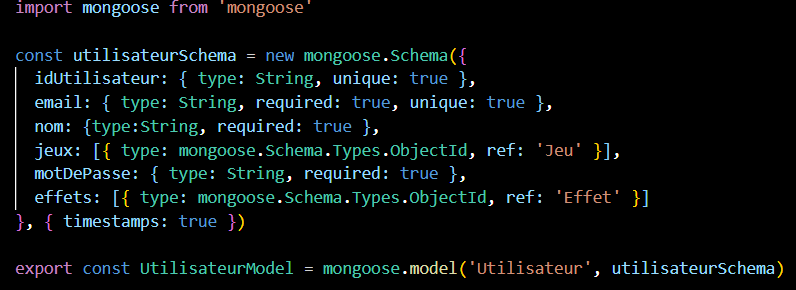
\includegraphics[width=\textwidth]{user.png}
    \caption{Création du schéma utilisateur}
    \label{fig:creation user}
\end{figure}

Ce code définit le modèle Mongoose Utilisateur utilisé dans le backend
pour représenter les comptes utilisateurs dans la base de données MongoDB.
Chaque utilisateur possède un idUtilisateur unique, un courriel, un nom
et un mot de passe.
Deux relations sont définies avec d'autres collections de la base de 
données: un tableau de références vers les jeux créés, 
lié à la collection Jeu, via des identifiants de type ObjectId, et 
un tableau de références vers des effets personnalisés, 
liés à la collection Effet.

\begin{figure}[H]
    \centering
    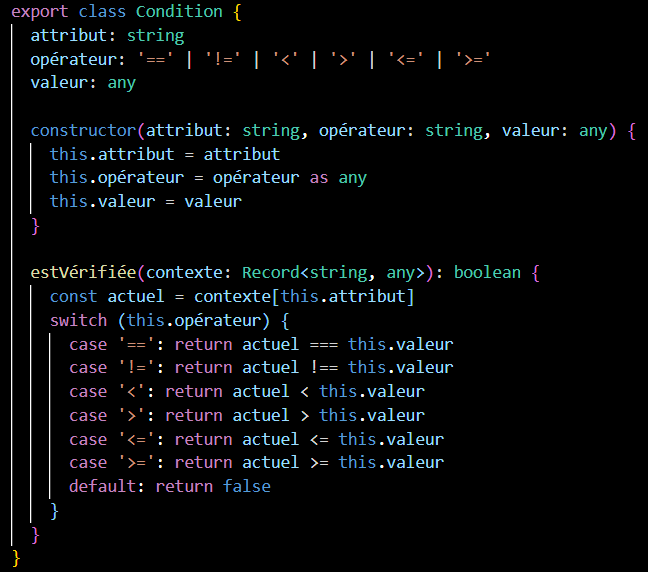
\includegraphics[width=\textwidth]{conditions.png}
    \caption{Conditions pour les jeux}
    \label{fig:conditions jeux}
\end{figure}

Ce code définit la classe Condition, utilisée pour représenter une 
condition logique dans le système d’effets du jeu. Chaque condition est 
composée d’un attribut, d’un opérateur (comme ==, !=, <, >=, etc.) 
et d’une valeur de comparaison. La méthode estVérifiée permet d’évaluer 
si la condition est remplie, en comparant dynamiquement la valeur d’un 
attribut dans un contexte donné (par exemple, les propriétés d’un joueur 
ou d’une case) avec la valeur cible. Le switch centralise tous les cas 
possibles d’opérateurs, ce qui rend cette classe facilement extensible 
et adaptée à l’exécution conditionnelle d’effets ou de règles dans le 
moteur de jeu.

\begin{figure}[H]
    \centering
    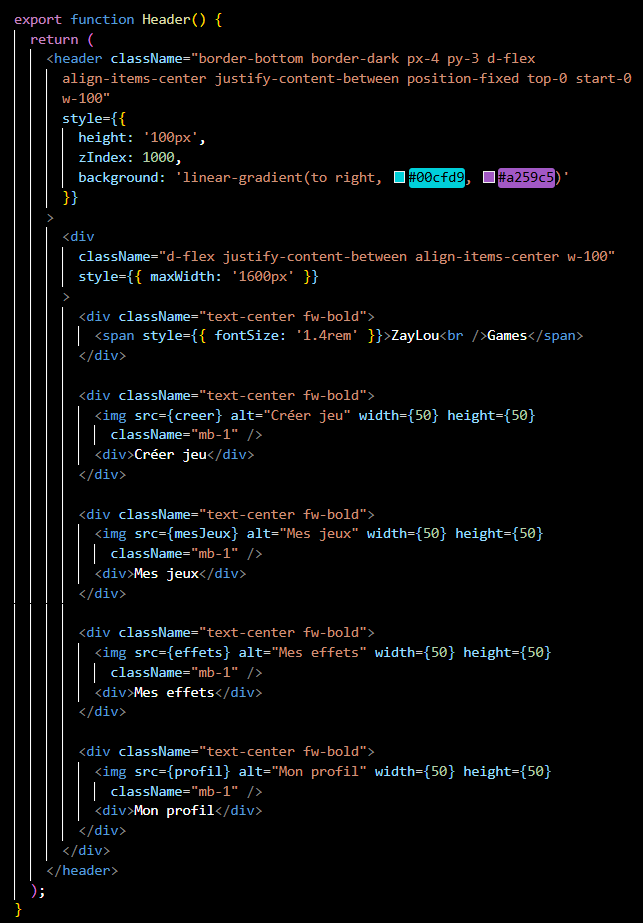
\includegraphics[width=\textwidth]{header.png}
    \caption{l'en tête de la plateforme}
    \label{fig:en tête plateforme}
\end{figure}

Ce composant React nommé Header définit l’en-tête de l’application 
ZayLou Games. Il utilise des classes Bootstrap pour assurer une mise en 
page responsive et bien alignée, avec une barre de navigation fixe en 
haut de l’écran. Le style inline applique un dégradé linéaire de couleur, 
ainsi qu’une hauteur et une priorité d’affichage.

\subsection{Captures d'écrans de l'application}
\label{subsec:Captures écran}

\begin{figure}[H]
    \centering
    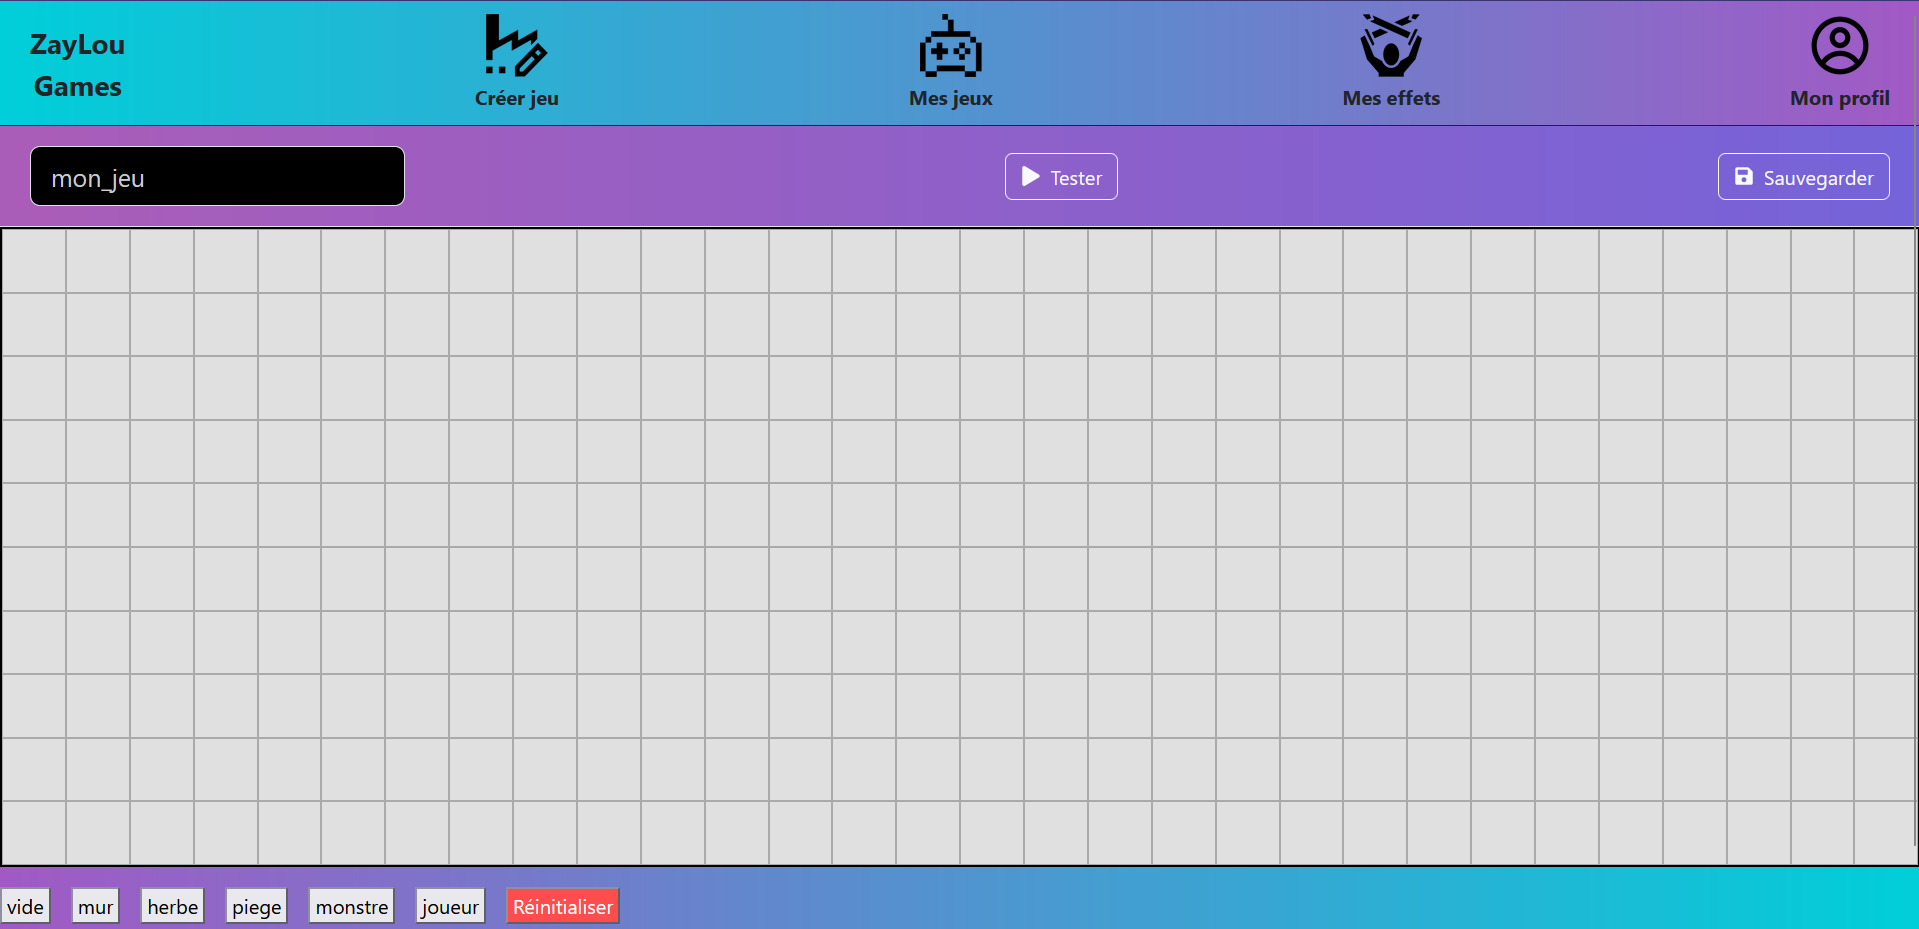
\includegraphics[width=\textwidth]{interface.png}
    \caption{Interface de la plateforme}
    \label{fig:interface de la plateforme}
\end{figure}

Cette capture d’écran montre l’interface principale de création de jeu 
dans l’application ZayLou Games. En haut, une barre de navigation fixe.
Juste en dessous, l’utilisateur peut nommer son jeu, lancer un test 
interactif via le bouton “Tester” (non implémenté) ou sauvegarder ses 
modifications avec le bouton “Sauvegarder”.

La partie centrale est occupée par une grille éditable, dans laquelle 
l’utilisateur peut construire la scène de son jeu. En bas, une palette 
d’outils permet de sélectionner le type de case à placer (vide, mur, 
herbe, piège, monstre, joueur), ou de réinitialiser entièrement la grille.

\begin{figure}[H]
    \centering
    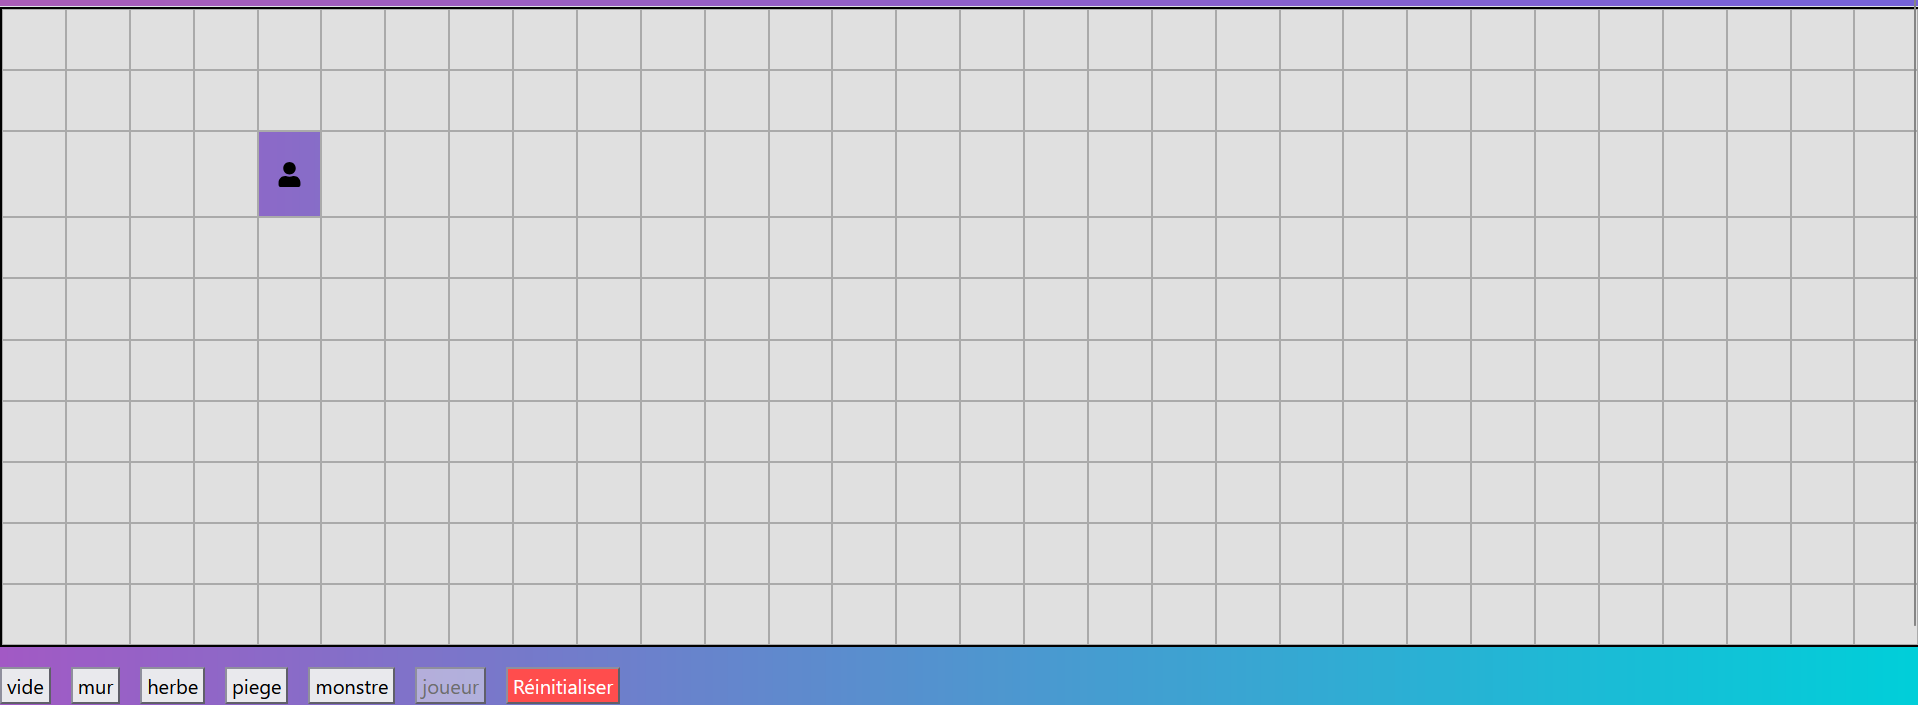
\includegraphics[width=\textwidth]{joueur.png}
    \caption{Grille avec case joueur}
    \label{fig:Grille avec joueurs}
\end{figure}

Cette capture d'écran présente la grille avec une case sélectionnée en 
tant que joueur. On voit aussi que le bouton pour sélectionner une case 
est désactivé. La plateforme ne permet pas que l'utilisateur définisse
joueurs dans la grille.

\subsection{Jeux de tests, résultats d’évaluation complets}
\label{subsec:Jeux de tests}

\subsection{Documentation technique, schémas supplémentaires}
\label{subsec:schémas supplémentaires}

\begin{figure}[H]
    \centering
    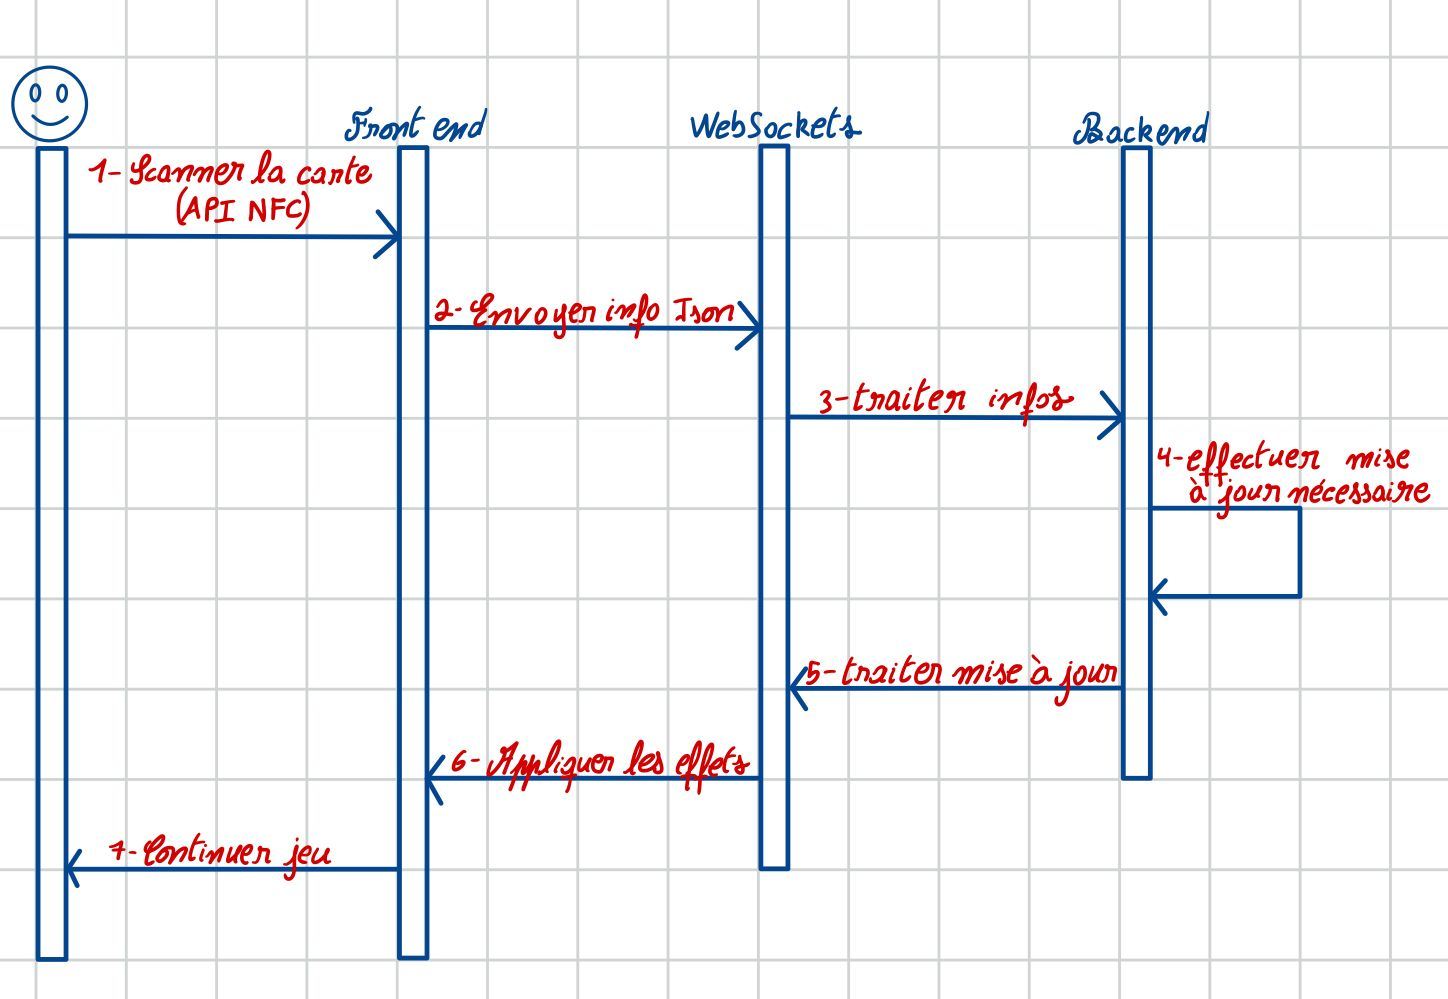
\includegraphics[width=\textwidth]{sequence_websocket.jpg}
    \caption{Diagramme de séquence avec WebSocket}
    \label{fig:Séquence WebSocket}
\end{figure}

Ce diagramme de séquence représente le processus de déclenchement d’un 
effet en temps réel suite au scan d’une carte NFC, via une communication 
WebSocket. Ce flux était initialement prévu pour les jeux en multijoueurs.



\end{document}                      % Fin du documents